% -*- encoding=utf-8 -*-
%!TEX program = xelatex
\documentclass[UTF8]{ctexart}

\usepackage{amsmath}
\usepackage{graphicx}
\DeclareGraphicsExtensions{.eps,.ps,.jpg,.bmp,.png}

\begin{document}

\begin{flushleft}
Titile: LSTM中文 \\
author: Ian \\
email: stmayue@gmail.com
\end{flushleft}

因为最近接触得比较多,所以一直想尝试一下LSTM的基本推导,从2000年《Learning to forget-Continual prediction with LSTM》这篇文章的模型入手,现在已经有了新的模型了,就是将cell的输出也连接到各个gate作为输入(peephole connection),如果后面有兴趣的话会完成这部分。

LSTM对于搞NLP的同学来说已经不陌生了,所以这里假设都对该模型有基本的了解,下面会给出必要的公式以及简要的前向过程,主要是对原文公式的详细推导和总结。

\begin{figure}[h!]
    \centering
    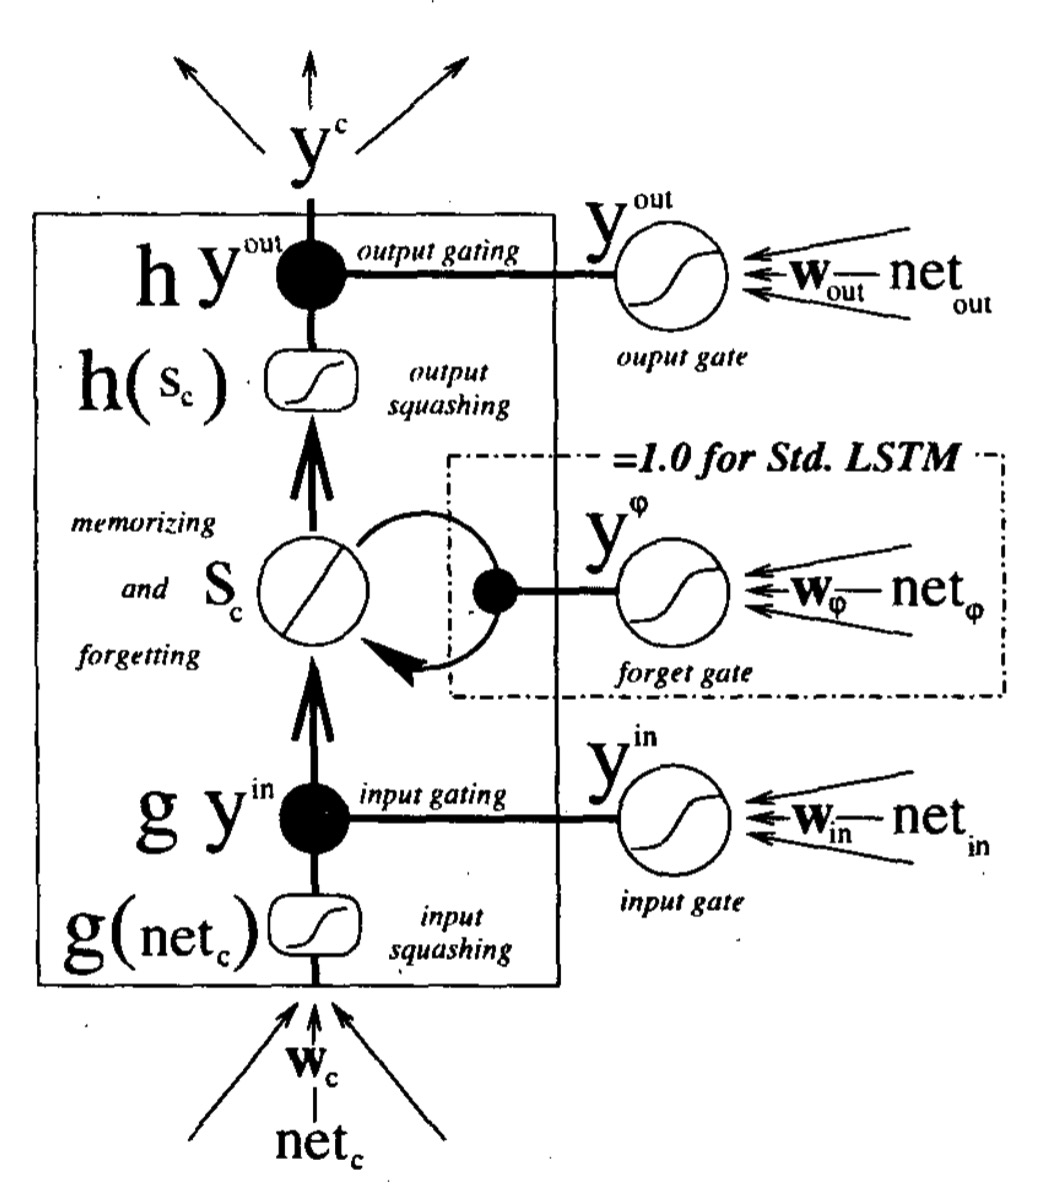
\includegraphics[width=10cm]{lstm.png}
    \caption{基本的LSTM}
    \label{fig-sample}
\end{figure}

图一给出了LSTM的基本模型,对于该模型,有以下几个计算过程.
对于一个memory cell从底部向上的计算过程为:
首先是计算各个子部分,包括net\_c, output gate, input gate, forget gate

% \begin{align}
% \end{align}

\begin{align}
net_{c^v_j}(t) &= \sum_m \, \omega_{c^v_{j}m} \, y_{m}(t-1) \\
y^{out_j}(t) &= f_{out_j}(\sum_m \, \omega_{out_{j}m} \, y_{m}(t-1)) \\
y^{in_j}(t) &= f_{in_j}(\sum_m \, \omega_{in_{j}m} \, y_{m}(t-1)) \\
y^{forget_j}(t) &= f_{forget_j}(\sum_m \, \omega_{forget_{j}m} \, y_{m}(t-1))
\end{align}

cell部分的计算为:
\begin{equation}
S_{C^v_j}(t) = y^{forget_j}(t) \, S_{c^v_j} + y^{in_j}(t) \, g(net_{c^v_j}(t))
\end{equation}

输出为:
\begin{equation}
y^{c^v_j}(t) = y^{out_j}(t) \, h(S_{c^v_j}(t))
\end{equation}

上述公式中$y$为每个节点的输出,$j$为第$j$个memory cell block,$v$为第$v$个memory cell,一般我们是一个block,memory cell产生的是标量,组合起来block产生的就是向量了。

公式$(1)-(4)$完成了一个memory cell的前向过程,为了使后向过程更方便计算,建立一个完整的模型,这里假设LSTM是一个hidden layer,上层接一个output layer,计算如下:

\begin{equation}
y^{k}(t) = f_{k}(\sum_v\omega_{kc^v_j} \, y^{c^v_j}(t))
\end{equation}

至此,前向过程已经过了一遍,对应的是利用上面的前向步骤来推导参数的误差,即学习过程。下面为反向的推导。

这里使用$\frac{1}{2}$平方误差来计算,有:
\begin{align}
E(t) &= \frac{1}{2}\sum_{k}e_k(t)^2 \\
e_k(t) &= t^k(t) - y^k(t)
\end{align}

和$y^k$最相关的是$\omega_{kc^v_j}$,那么它的权值更新可以通过下面公式计算而来:

\begin{align}
\delta_k(t) &= {f'}_{k}(net_k (t)) \, e_k(t) \\
net_k(t) &= \sum_v \, \omega_{kc^v_j} \, y^{c^v_j}(t) \\
\Delta \omega_{kc^v_j} &= \alpha \, \delta_k(t) \, y_{c^v_j}(t)
\end{align}

接下来,可以看到$y^{c^v_j}(t)$直接和$y^{out_j}(t)$相关,可以先求output gate的误差,通过一系列展开式来说明:

\begin{align}
y^{k}(t) &= f_k(\sum_v \omega_{kc^v_j} \, y^{c^v_j}(t)) \\
&= f_k(\sum_v \omega_{kc^v_j} \, y^{out_j}(t) \, h(S_{c^v_j}(t)))
\end{align}

通过链式法则分步来求其偏导数,可得

\begin{align}
\frac{\partial E(t)} {\partial y^k(t)} &= e_k(t) \\
\frac{\partial y^k(t)} {\partial y^{out_j}{t}} &= {f'}_k(net_k(t)) \, \sum_v\omega_{kc^v_j} \, h(S_{c^v_j}(t)) \\
\frac{\partial y^{out_j}(t)} {\partial \omega_{out_j}} &= {f'}_{out_j}(net_{out_j}(t)) \, y^m(t-1) \\
\end{align}

连乘并考虑output layer的$k$个输出可得

\begin{align}
\delta_{out_j}(t) &= \sum_k e_k(t) \, {f'}_k(net_k(t)) \, \sum_v\omega_{kc^v_j} \, h(S_{c^v_j}(t)) \, {f'}_{out_j}(net_{out_j}(t)) \\
&= {f'}_{out_j}(net_{out_j}(t)) \, (\sum_v h(S_{c^v_j}(t)) \, \sum_k\omega{kc^v_j} \, \delta_k(t)) \\
\Delta \omega_{out_j} &= \alpha \, \delta_{out_j} \, y^m(t-1)
\end{align}

接下来求input gate,forget gate以及最底层输入$(\omega_{c^v_j})$计算的误差,可以看出,这几个参数只和$S_{c^v_j}$有关,在这之前的误差传播对于这三个都是一样的,我们使用$e_{s_{c^v_j}}$来统一表示,从上面公式(6)以及(20)可以得到

\begin{equation}
e_{s_{c^v_j}} = y^{out_j}(t) \, {h'}(S_{c^v_j}(t)) \, (\sum_k\omega_{kc^v_j} \, \delta_k(t))
\end{equation}

重新看一下公式(5),为

\begin{equation*}
S_{C^v_j}(t) = y^{forget_j}(t) \, S_{c^v_j} + y^{in_j}(t) \, g(net_{c^v_j}(t))
\end{equation*}

根据上面的式子来求导数,那么对于input gate,有

\begin{equation}
\frac{\partial S_{c^v_j}(t)} {\partial \omega_{in_j}} = \frac{\partial S_{c^v_j}(t-1)} {\partial \omega_{in_j}} \, y^{forget_j}(t) + g(net_{c^v_j}(t)) \, {f'}_{in_j}(net_{in_j}(t)) \, y^m(t-1)
\end{equation}

对于forget gate,公式(5)只有加号前面的一下和其有关,按照分部积分原则,有

\begin{equation}
\frac{\partial S_{c^v_j}(t)} {\partial \omega_{forget_j}} =  \frac{\partial S_{c^v_j}(t-1)} {\partial \omega_{forget_j}} \, y^{forget_j}(t) + S_{c^v_j}(t-1) \, {f'}_{forget_j}(net_{forget_j}(t)) \, y^m(t-1)
\end{equation}

对于$(\omega_{c^v_j})$,有

\begin{equation}
\frac{\partial S_{c^v_j}(t)} {\partial \omega_{c^v_j}} =  \frac{\partial S_{c^v_j}(t-1)} {\partial \omega_{c^v_j}} \, y^{forget_j}(t) + g'(net_{c^v_j}(t)) \, y^{in_j}(t) \, y^m(t-1)
\end{equation}

上述公式中,涉及$S_{c^v_j}(t-1)$的偏导数都能在上一时刻的计算中求得,并且在$t = 0$时刻均初始化为0。此外涉及$g, f$的求导的部分,依据所选用的激活函数来计算,假设使用了sigmoid的函数,那么有
\begin{equation}
f'(x) = x \, (1-x)
\end{equation}

基本的LSTM推导完成。

\end{document}

